\chapter{Mechanical Design}

Unless the chapter heading already makes it clear, an introductory paragraph that explains how this chapter contributes to the objectives of the report/project.

\section{Extruder Design}
\subsection{Concept Generation}
\subsubsection*{Concept 1}
\begin{figure}[H]
    \centering
    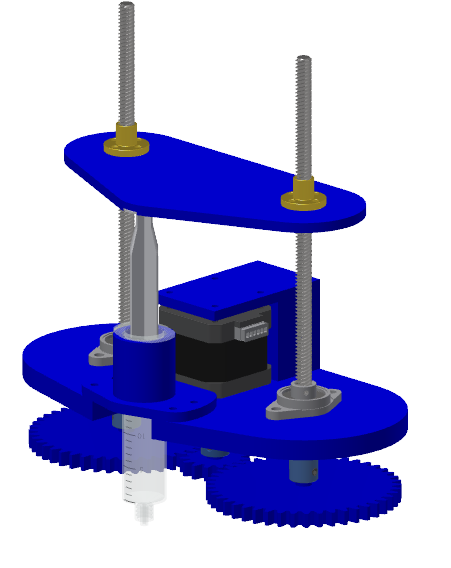
\includegraphics[scale=1]{figs/SyringeConcept1.png}
    \caption{Concept 1 Syringe-Based Extruder}
    \label{fig:extruderConcept1}
\end{figure}
\subsubsection*{Concept 2}
\begin{figure}[H]
    \centering
    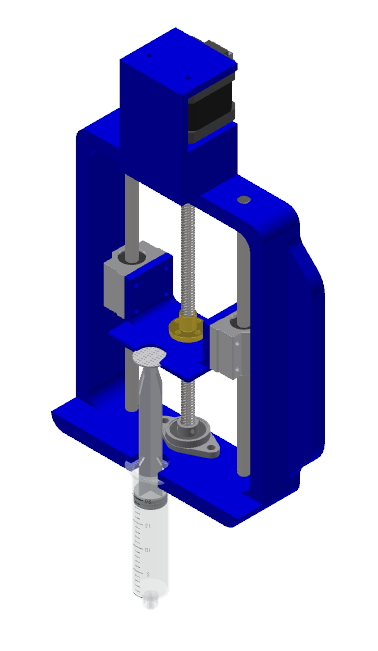
\includegraphics[scale=1]{figs/SyringeConcept2.png}
    \caption{Concept 2 Syringe-Based Extruder}
    \label{fig:extruderConcept2}
\end{figure}
\subsubsection*{Concept 3}
\begin{figure}[H]
    \centering
    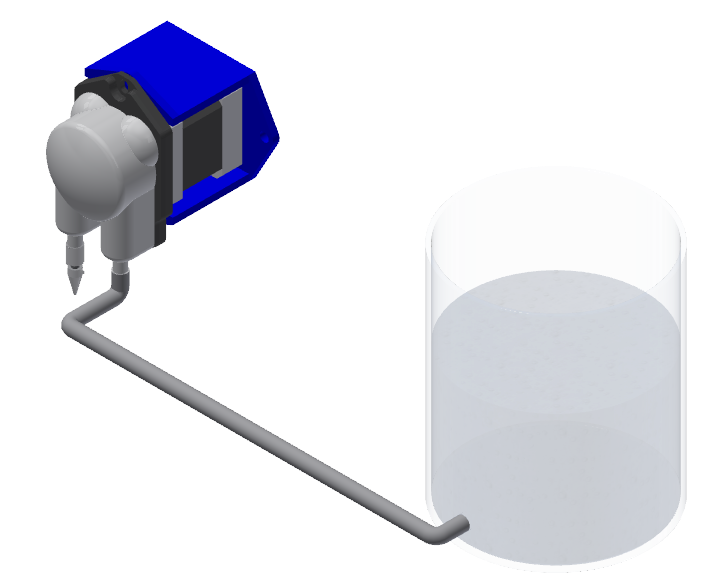
\includegraphics[scale=1]{figs/PumpConcept.png}
    \caption{Concept 3 Pump-Based Extruder}
    \label{fig:extruderConcept3}
\end{figure}
\subsection{Concept Evaluation and Selection}
\subsection{Final Design}


\section{Gantry Design}
\subsection{Concept Generation}
\subsubsection*{Concept 1}
\subsubsection*{Concept 2}
\subsection{Concept Evaluation and Selection}
\subsection{Final Design}


\section{Final Assembled Bioprinter}